\subsection{Fachgruppe bzw. Fachgruppenrat}
\label{fachgruppe}

Die Fachgruppe Informatik besteht eigentlich aus allen 
Informatikstundenten, also ab jetzt auch aus euch. Der Fachgruppenrat 
ist die studentische Vertretung f"ur Studierende der Informatik, also 
eine Art "`Jahrgangssprecher"', die jedes Semester von euch gew"ahlt werden 
und als Bindeglied zwischen den Studierenden und dem Fachbereich 
fungieren. Oft wird aber auch einfach "`Fachgruppe"' gesagt, wenn man 
eigentlich vom "`Fachgruppenrat"' spricht - vielleicht auch deshalb, 
weil wir keinen großen Wert auf eine Trennung legen, sondern das ganze
eher als fließenden Übergang zwischen viel und wenig Engagement sehen.

Unsere Hauptaufgabe ist die Vertretung eurer und unserer Meinung 
gegen"uber der Fakult"at in verschiedenen Kommissionen. Kommissionen 
gibt es an der Uni zuhauf, um die verschiedensten Angelegenheiten zu 
regeln. Ein Beispiel ist etwa die Studienkommission, in der ständig 
an den Studienabschl"ussen Bachelor und Master gefeilt wird. Den Bachelor 
gibt es zwar inzwischen schon seit einigen Jahren, aber dank des 
Bildungsstreiks in den Jahren 2009/2010 gibt es nun eine ganze Reihe % TODO mit etwas Glück wird es noch einen Artikel zum Bildungsstreik geben, der dann von hier aus verlinkt werden sollte
von neuen (hoffentlich besseren) Regelungen, die eingearbeitet werden 
müssen.

Zus"atzlich versuchen wir, euch bei Fragen und Problemen rund um das 
Studium weiterzuhelfen. Besonders allen Erstsemestern stehen wir 
gerne mit Rat und Tat zur Seite.  Mehr dazu im Abschnitt ,,Termine'' auf
Seite \pageref{termine}.
%Es gibt zwei Einfühungstermine, an denen wir euch einiges rund um die 
%Uni erz"ahlen m"ochten: ??????

\subsubsection*{FG-Blog}

Auf unserer Webseite \url{http://fginfo.cs.tu-bs.de} seht ihr nicht 
nur, welche Schwerpunkte wir gerade bei unserer Fachgruppenarbeit setzen, 
sonder ihr werdet auch "uber aktuelle Veranstaltungen informiert, und k"onnt 
die Erstsemesterzeitung (die ihr gerade in Händen haltet), herunterladen. 
Am besten abonniert ihr unseren RSS-Feed, dann bekommt ihr automatisch 
mit, wenn es etwas neues gibt.

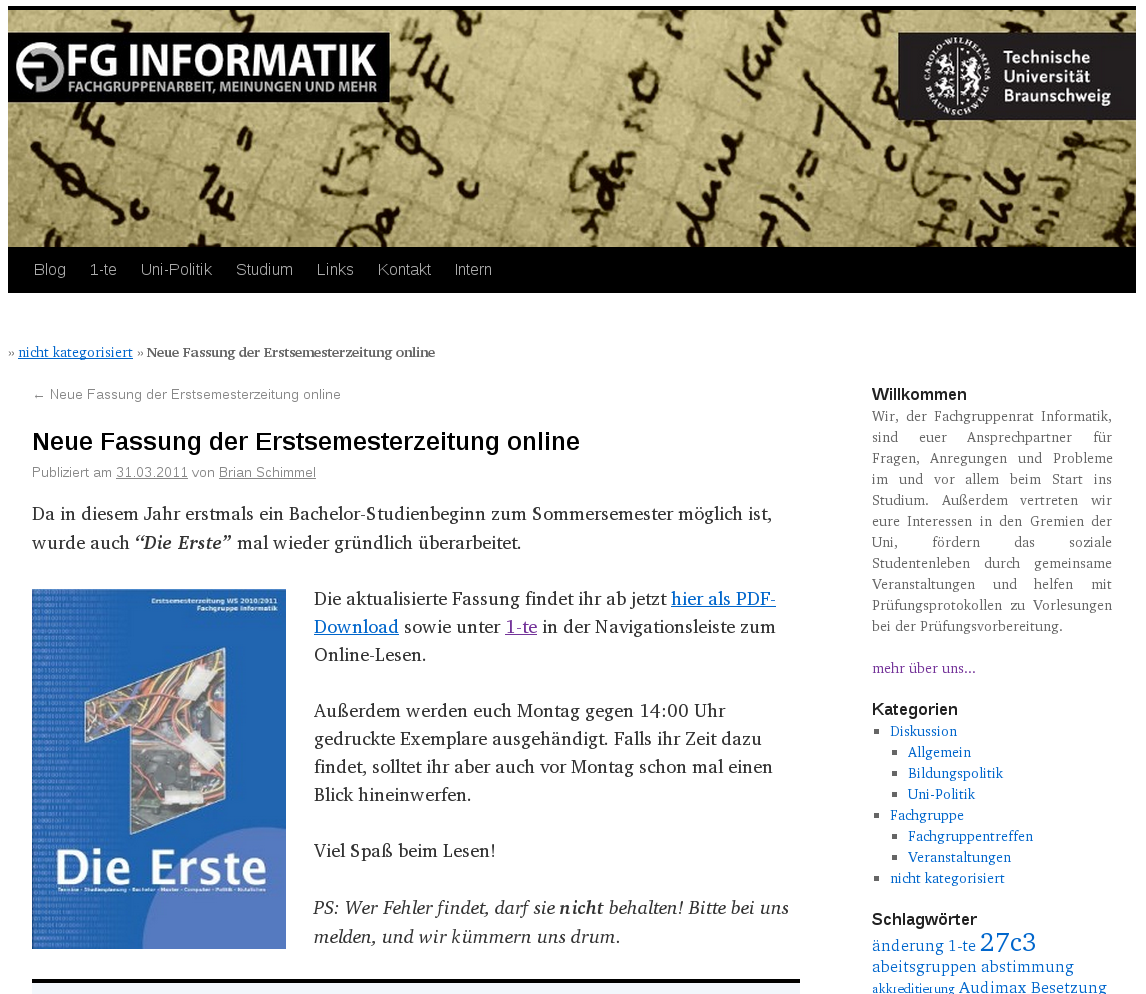
\includegraphics[width=\columnwidth]{bilder/fgblog.png}

Wenn ihr uns persönlich Fragen ansprechen wollt, kommt 
in unsere regelmäßige Sprechstunde, oder zum wöchentlichen Fachgruppentreffen.
Die konkreten Termine standen bei Drucklegung noch nicht fest, aber ihr könnt
sie auf unserem oben genannten Blog nachlesen. Wir haben praktisch immer wichtige 
Neuerungen zu diskutieren und suchen permanent Unterstützung und 
Nachwuchs. Ab und zu beim Fachgruppentreffen herein zu schauen ist 
nicht nur der perfekte Einstieg, um sich selbst einmal einzubringen, 
sondern gibt euch euch die Möglichkeit, immer auf dem neuesten Stand 
der Entwicklungen zu bleiben, die euch letztlich selbst betreffen werden.
